\documentclass[runningheads]{llncs}
\usepackage{graphicx}
\usepackage{filecontents,lipsum}
\usepackage[noadjust]{cite}
\usepackage{amssymb}
\usepackage{amsmath}
\usepackage{array}
\usepackage{multirow}
\usepackage{footnote}
\usepackage{cases}
\usepackage{listings}
\usepackage{booktabs}
\usepackage{tabularx}
\usepackage{float}
\usepackage{tikz}
\usepackage{tabularx}
\usepackage[flushleft]{threeparttable}

\usepackage{lipsum}
\usepackage{capt-of}
\usepackage{tikz}
\usepackage{scrextend}
\usepackage{mathrsfs}
\usetikzlibrary{arrows}
\usepackage{epsfig}	
\usepackage{booktabs}
\usepackage{caption}
\usepackage{subcaption}
\usepackage{breqn}
\usepackage{array}

\newcolumntype{P}[1]{>{\centering\arraybackslash}p{#1}}
\newcolumntype{M}[1]{>{\centering\arraybackslash}m{#1}}


\DeclareGraphicsExtensions{.pdf,.jpeg,.png,.tif}
\makeatletter
\def\BState{\State\hskip-\ALG@thistlm}
\usepackage[figuresright]{rotating}	

\setcounter{secnumdepth}{5}
\setcounter{tocdepth}{5}
\usepackage{xcolor}
\usepackage{color, colortbl}
\usepackage[linesnumbered,ruled,vlined]{algorithm2e}
\newcommand\mycommfont[1]{\footnotesize\ttfamily\textcolor{blue}{#1}}
\SetCommentSty{mycommfont}
\usepackage{algcompatible}
\usepackage[ruled,vlined]{algorithm2e}
\usepackage{algpseudocode}




\definecolor{Gray}{gray}{0.4}
\usepackage[pagebackref=false,breaklinks=true,letterpaper=true,colorlinks,bookmarks=false]{hyperref}

\usepackage[utf8]{inputenc}
\usepackage[english]{babel}
%\usepackage{amsthm}
%\theoremstyle{definition}
% \newtheorem{definition}{Definition}[section]
%\theoremstyle{remark}
%\newtheorem*{remark}{Remark}
\setlength{\fboxsep}{0pt}



\begin{document}

\title{Background Removal of French University Diplomas}

\author{Tanmoy Mondal\inst{1} \and Quoc Bao Dang\inst{2} \and Mickaël Coustaty\inst{2} \and Petra Gomez-Krämer\inst{2}\and Jean-Marc Ogier\inst{2}}

\authorrunning{T. Mondal et al.}

\institute{Zenith, INRIA, Montpellier, France \and
L3i, University of La-Rochelle, France \\
\email{ tanmoy.mondal@inria.fr, \{quoc\_bao.dang,  petra.gomez, mickael.coustaty, jean-marc.ogier\}@univ-lr.fr}  }
%
\maketitle              % typeset the header of the contribution
%
\begin{abstract}
		Separation of foreground text from noisy or textured background is an important preprocessing step for many document image processing problems. In this work we focus on decorated background removal and the extraction of textual components from French university diploma. As far as we know, this is the very first attempt to resolve this kind of problem on French university diploma images. Hence, we make our dataset public for further research, related to French university diplomas. Although, this problem is similar to a classical document binarization problem but we have experimentally observed that classical and recent state of the art binarization techniques fails due to the different complexity of our dataset. In French diplomas, the text is superimposed on decorated background and there is only a small difference of intensities between the character borders and the overlapped background. So, we propose an approach for the separation of textual and non-textual components, based on Fuzzy-C-Means clustering. After obtaining clustered pixels, a local window based thresholding approach and the Savoula binarization technique is used to correctly classify pixels, into the category of text pixels. Experimental results show convincing accuracy and robustness of our method.  

\keywords{Text-Graphics Separation \and French University Diplomas \and Document Binarization \and Fuzzy C-Means Clustering.}
\end{abstract}


	\section{Introduction}
\label{intro}
Separation of text foreground from page background is an important processing step for the analysis of various kind of documents e.g. historical, administrative, scanned and camera captured documents. This separation enables various document analysis algorithms (such as character recognition, localization of stamps, logos, signatures etc.) to focus only on the written text without the disturbing background noise. If texts and graphics are located in separate regions in the page, localizing the region of texts and graphics is easier in comparison with texts superimposed on background graphics \cite{Ahmed2012a}.

In this paper, we are focusing on the proper extraction of all the text components from French university diploma, which contains a complex background. The objective is to secure university diploma and to reduce the possibilities of fraud. The core idea is to encode a unique and secret number in the diploma while printing it. This encoding is done by changing the shape of certain characters and each modified character shape is associated with a specific digit (this association is only known to some specific people of the university). Hence, later to check the authenticity of any scanned student's diploma, we need proper and un-deformed extraction of text characters which is required for decoding the secret and unique number, associated with each diploma. 
All French university diplomas are printed on the same decorated and authenticate thick paper/parchment (in French called as : \textit{parchemin}), only and strictly fabricated by the National Printing House (in French called as: \textit{Imprimerie Nationale}). 
So, any French university diploma has the same background and only the foreground text changes for different universities/institutes (moreover scanned diploma will diversify due to scanning effects). Moreover, the text fonts, size and text styles also varies for different universities/institutes. In every diplomas, each individual student's information e.g. name, date-of-birth, place-of-birth etc. changes also. All these variation together, makes the binarization process harder.  
%	The objective is to verify the authenticity of student diplomas e.g. for job, university application etc.
% Students can send the scanned copy of their diplomas in color or gray scale format, depending on the configuration of the used scanners. 
%	Any pragmatic approach of subtracting one sample background won’t work as different scanned diploma image can have variable backgrounds due to the variation in condition/settings/environmental effects during scanning process (that’s why, we intentionally avoided to use any color information for our algorithm).  
This complex background is highly superimposed with the foreground textual components which makes it complex to separate the textual components from the background (see Fig. \ref{image_text_0} for an example of diploma). This problem can also be seen as separation of graphical background from the textual foreground. On the other hand, this problem has a high resemblance with historical degraded document binarization. Historical degradation includes non-uniform background, stains, faded ink, ink bleeding through the page and un-even illumination \cite{Bataineh2011}.  
%	A Proper extraction of the texts is needed for further text based processing of the diplomas, such as character recognition, localization of stamps, logos, signatures etc. The graphics recognition community has already put a lot of effort into research on text/graphics segmentation. 
%	In general, different methods have been proposed to perform text/graphics segmentation in different scenarios. 
%	In document images, mostly parts of text overlap with graphics. To extract the overlapping text is an important challenge in text/graphics segmentation and is still an open problematic domain \cite{Biswas2014}. 
The state of the art text-graphics separation approaches do not perform well in our case because unlike general text-graphics separation data e.g. maps, floor plans etc. \cite{Ahmed2012a}, the texts in diploma images are fully superimposed upon the decorated colored background. 

There exist several categories of binarization techniques, which are often evaluated on the dataset of popular document image binarization contest (DIBCO) \cite{Pratikakis2018}. But these categories of binarization approaches have several constraints. Many common binarization approaches are based on the calculation of local or global thresholds and image statistics, which doesn't work for our case (see experimental section in \ref{results}). So as a contribution of this paper, we propose a new algorithm for the separation of text components from graphical background. 
The algorithm starts by structured forest based fast gradient image formation followed by textual region selection by using image masking for the initial filtering of textual components. Then Fuzzy-C-Means clustering is applied to separate textual and non-textual components. As the clustering may result in some deformation of the textual components (characters), hence we also propose character reconstruction technique by using a local window based thresholding approach and Savoula binarization algorithm \cite{Sauvola2000}. This technique helps to correctly classify some extra pixels into the category of text pixels, which helps to reconstructs/recover the missing character pixels. As far as we know, this is the very initial proposed attempt of removing background to obtain texts from French university diplomas.
%	In our experiments, we have obtained accuracy ($F-Measure$) of 93\% (approx.) on total $40$ diploma images. Moreover, we also shown the applicability of proposed method, designed for diploma datasets on classical problem binarization on DIBCO dataset \cite{Pratikakis2018}

The remainder of this paper is organized as follows. First, Section II summarizes the work related to text/graphics
segmentation in general. Then, Section III provides an overview of the method proposed. Subsequently, experimental results are described and analyzed in Section IV. Finally, Section V concludes the paper and gives an overview of future work.
\begin{figure}[h!]	       
	\centering
	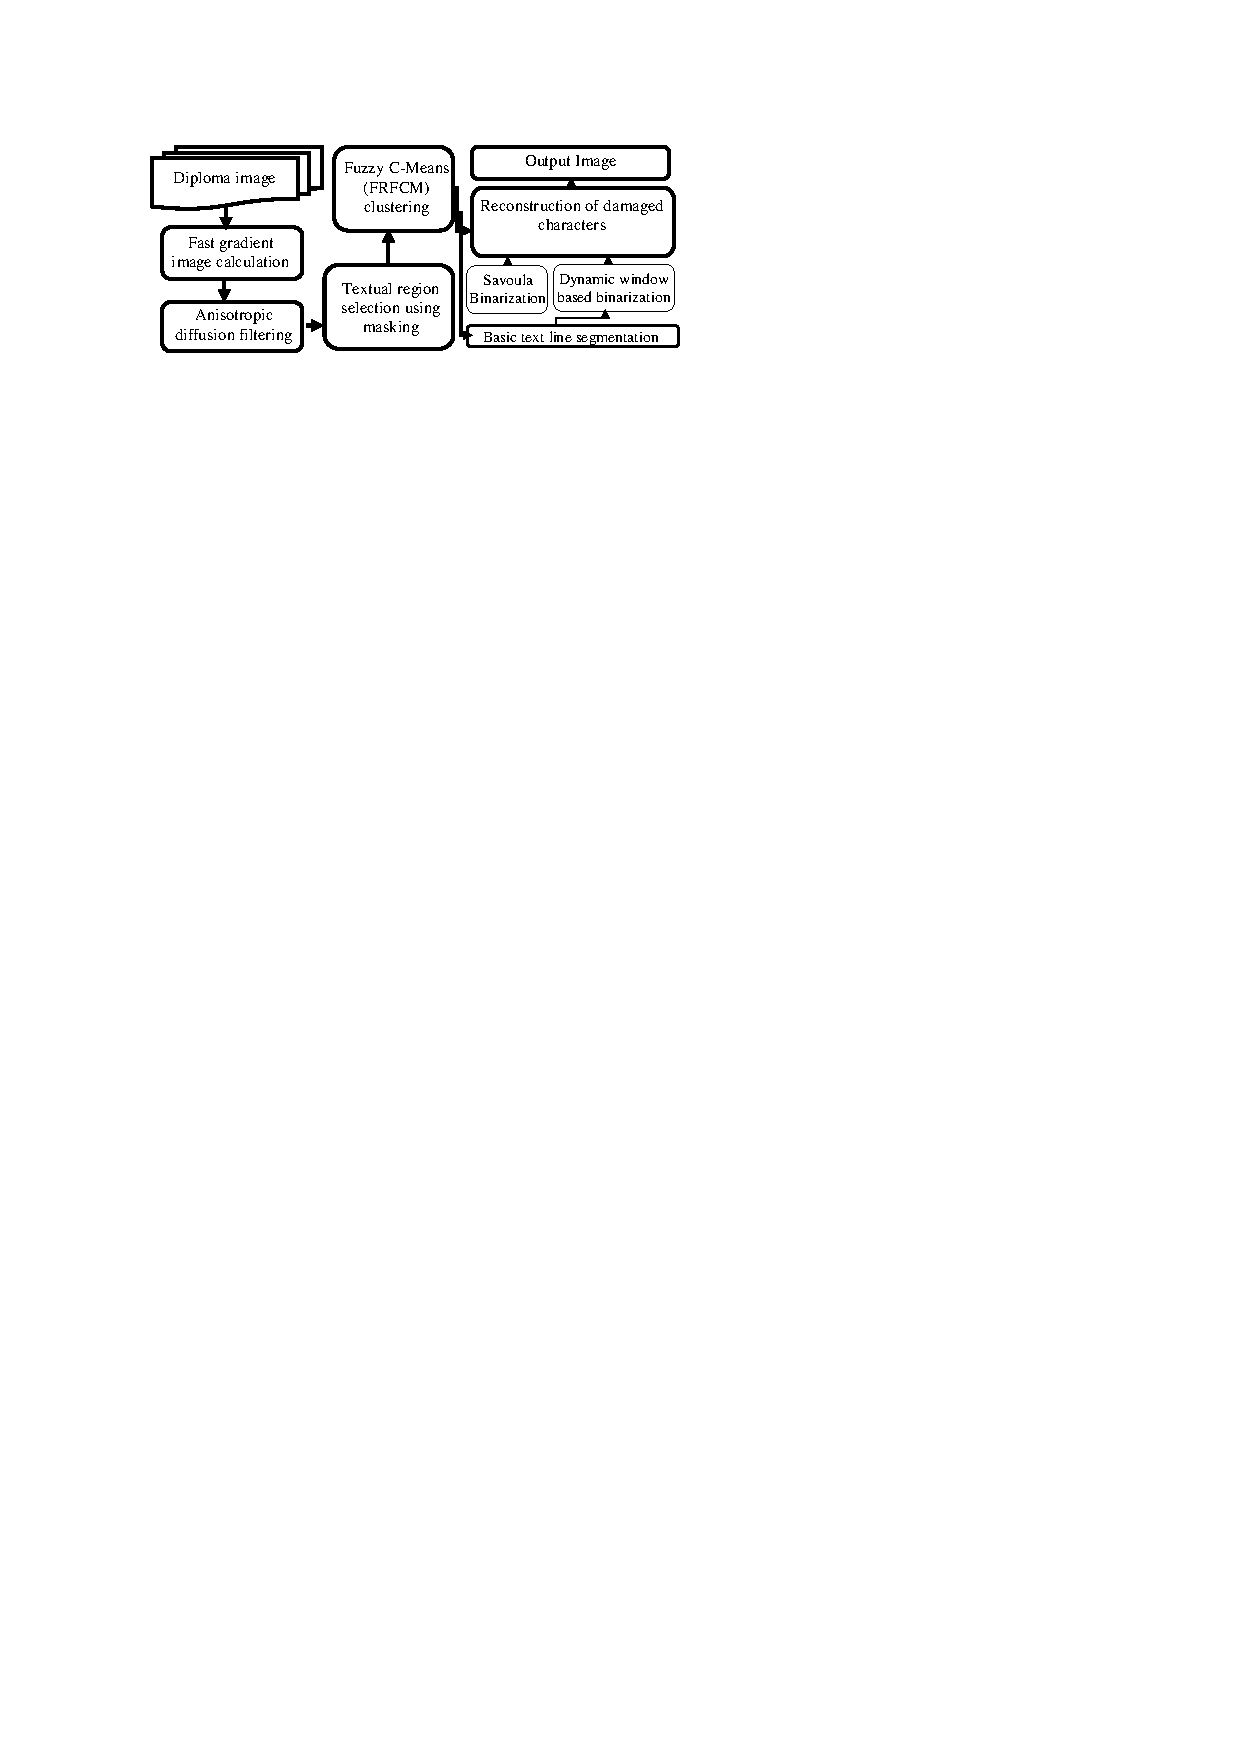
\includegraphics[trim = 2.4cm 23.6cm 9.5cm 2.3cm, clip,  scale = 0.95]{./images/schema}
	\caption{The proposed algorithm architecture. The portions in bold are the main steps of the algorithm while the two non-bold blocks are the auxiliary steps needed for the \textit{"reconstruction of damaged character"}block}.  
	\label{fig:architecture}
\end{figure}
	\section{Related Work}
\label{related_work}
By definition, text binarization means the labeling of each pixel in the image as text or background which has a good resemblance with our problem. Due to the unavailability of any previous work, we have outlined here some of the related work from the domain of document image (mainly historical) binarization. The existing binarization techniques in the literature can be categorized into two principal categories: learning-free and learning-based approach. Several binarization techniques have been proposed in the past decade but very recently the trend in document binarization tends to machine learning based methods, mostly relying on deep-learning based techniques. 

Most deep learning based image binarization algorithms use convolutional neural network (CNN), e.g. by Tensmeyer and Martinez \cite{Tensmeyer2018}, or variations thereof, such as the deep supervised network (DSN) approach proposed by Vo et al. \cite{Vo2017}.  
%	Westphal et. al \cite{Westphal2018} proposed a recurrent neural networks (RNNs) with long short-term memory (LSTM) cells based technique for image binarization. 
Due to the requirement of sufficient amount of training data and specially in our case, where no ground truth exists, the training based approaches are not useful. Moreover, recently the learning-free approaches \cite{Jia2016} have shown high potential and comparable accuracy with respect to learning-based approaches. In \cite{Bataineh2011}, a local binarization method based on a thresholding with dynamic and flexible windows is proposed. Jia et al. \cite{Jia2016} proposed an approach based on structural symmetry of pixels (SSP) from text strokes for binarization. Using the combination of SSP and Fuzzy C-Means (FCM) clustering (the FRFCM technique \cite{Lei2017}), Mondal et al. \cite{Mondal2019} also proposed an improved and fast binarization technique for historical document images. 

While Deep Learning methods is getting more and more attention in the community, FCM \cite{Lei2017} based models are among the popularly used methods for image segmentation. We avoided to use any learning based methods (e.g. deep neural networks) for background removal due to the non availability of pixel's level ground truth (GT). It is also highly cumbersome and expensive to generate such GT for our high resolution experimental data set. These methods rely on the Fuzzy set theory which introduce fuzziness for the belongingness of each image pixels in certain class. Such clustering technique, named as (FRFCM) \cite{Lei2017} , is used as one of the main processing step for our proposed algorithm. So, here we also provide a brief background and state of the art methods on FCM techniques to justify our choice.
%	As mentioned earlier that we use a fast Fuzzy C-Means clustering technique, named as (FRFCM) \cite{Lei2017} is used as one of the main processing step for our proposed algorithm. So, here we also provide a brief background and state of the art methods on FCM techniques to justify our choice.
%	Based on Fuzzy set theory, Fuzzy C-Means (FCM) \cite{Lei2017} is one of the most used methods for image segmentation and its success is highly attributed thanks to the introduction of fuzziness for the belongingness of each image pixels in certain class. 
It is superior to hard clustering as it has more tolerance to ambiguity and retains better original image information. 
As FCM only considers gray-level information without considering the spatial information, it fails to segment images with complex texture and background or images corrupted by noise. So, the FCM algorithm with spatial constraint (FCM\_S) \cite{Lei2017} was proposed, which incorporates spatial information in the objective function. However, FCM\_S is time consuming because the spatial neighbor term is computed in each iteration.
To reduce the execution time, two modified versions, named as FCM\_S1 and FCM\_S2 \cite{Lei2017} were proposed. These algorithms employ average filtering and median filtering to obtain the spatial neighborhood information in advance. However, both FCM\_S1 and FCM\_S2 are not robust to Gaussian noise, as well as to a known noise intensity.

The Enhanced FCM (EnFCM)\cite{Lei2017} algorithm is an excellent technique from the viewpoint of low computational time as it performs clustering based on gray level histograms instead of pixels of summed image. 
However, the segmentation results by EnFCM is only comparable to that produced by FCM\_S. To improve the segmentation results, the Fast Generalized FCM (FGFCM) \cite{Lei2017} was proposed. It introduces a new factor as a local similarity measure, which guarantees both noise immunity, detailed preservation of image segmentation. 
Along with that it also removes the requirement of empirical parameter $\alpha$ in EnFCM and performs clustering on gray level histograms. But FGFCM needs more parameter settings than EnFCM. 
A robust fuzzy local information C-Means clustering algorithm (FLICM) is introduced in \cite{Lei2017}, which is free from parameter selection. This algorithm replaces the parameter $\alpha$ of EnFCM by incorporating a novel fuzzy factor into the objective function to guarantee noise immunity and image detail preservation. Although FLICM overcomes the image segmentation performance but the fixed spatial distance is not robust to different local information of images. 
Hence, we use a significantly fast and robust algorithm based on morphological reconstruction and membership filtering (FRFCM) \cite{Lei2017} for image segmentation.
%	 proposed by Lei and Jia et al.\cite{Lei2017} (see in Section \ref{FRFCM} for the comparison with above mentioned state of the art Fuzzy C-Means clustering techniques).  

The aforementioned state of the art binarization methods are developed for the binarization of historical document images, by testing some of them, we observe unsatisfying results. In the following section, we propose a new method for separating the textual foreground from textured background.  
\section {Proposed Method}
In this section, the proposed algorithm is explained and it's overall architecture is shown in Fig. \ref{fig:architecture}. At first, the structural random forest based gradient image formation technique is applied on the image $\mathcal{I}(x,y)$ (see Fig. \ref{image_text_0}). 
\subsection {Structural Forest Based Fast Gradient Image Formation} \label{structuralForest} A real time gradient computation for the objective of edge detection is proposed by Dollár et al. \cite{Dollar2013}, which is faster and more robust to texture presence than current state of the art approaches; e.g. sobel \cite{Dollar2013}. The gradient computation (see Fig. \ref{image_text_2}) is performed based on the present structure in local image patches and by learning both an accurate and computationally fast edge detector. 

\subsection {Anisotropic Diffusion Filtering} \label{anisotropicDiff} 
	An anisotropic diffusion \cite{Gerig1992} filter is applied on the gradient image (see Section~\ref{structuralForest}) to reduce image noises (appears due to scanning) without removing significant contents of the image; e.g. edges, lines and other details (see Fig. \ref{image_text_3}). 
%	It produces a family of parameterized images, but each resulting image is a combination between the original image and a filter that depends on the local content of the original image. 

\subsection {Selection of Textual Regions from Original Image} \label{textualRegion} After filtering the image, edges are detected by the Canny edge detector (see Fig. \ref{image_text_4}). Only better gradient images are obtained by Dollár et al. \cite{Dollar2013} (refer to Section~\ref{structuralForest}) but to generate the binary edges, we have applied Canny edge detection algorithm.    
%	The threshold for canny edge detection is automatically computed by Otsu's global thresholding technique. 
The high and low threshold of Canny are computed automatically as $\phi$ (equal to Otsu's threshold value) and $0.5 \times \phi$. The idea was not to use hand-crafted thresholds.

The edge image is then dilated by using a $7 \times 7$ \footnote{Considering the high image resolution, we choose $7\times7$ kernel size. However, this parameter should be adapted to fit other dataset requirements.} rectangular kernel to connect the broken edges, caused by the Canny algorithm (see Fig. \ref{image_text_5}). It can be observed that it contains holes and gaps inside the character shapes (see Fig. \ref{image_text_5}). These holes/gaps are filled by applying the well known flood fill\footnote{\url{https://docs.opencv.org/2.4/modules/imgproc/doc/miscellaneous_transformations.html?highlight=floodfill}} based hole filling approach (see Fig. \ref{image_text_6}). Let us denote this hole filled image as $\mathcal{H}(x,y)$. 
Now original gray scale image pixels from the gray scale image corresponding to this hole filled image are simply obtained  by creating a blank image of the same size as the original image and initialized by 255 (let's say $\mathcal{T}(x,y)$; see Fig. \ref{image_text_7})). 
%	Now, if any pixel is a foreground pixel in $\mathcal{H}(i,j)$ (image background is white (255) and foreground in black (0)) then the same pixel is copied from the original gray scale image ($\mathcal{I}(x,y)$) and put into $\mathcal{T}(x,y)$). 
This process corresponds to applying a mask\footnote{background is white (255) and foreground is black(0)} using image $\mathcal{H}(x,y)$. Now a clustering technique is applied to the masked image $\mathcal{T}(x,y)$ for classifying the text pixels from the background pixels. 
\begin{equation}
\mathcal{T}(x,y) =
\begin{cases}
\mathcal{I}(x,y); & \text{if $\mathcal{H}(x,y)$ = 0}.\\
255; & \text{otherwise}.
\end{cases}
\end{equation}	 

\begin{figure*}[h]
	\centering
	\begin{subfigure}[b]{0.4\textwidth}
		\centering\includegraphics[trim = 0cm 1cm 0cm 0cm, clip,scale=0.018]{./images/1_original_Image.jpg}
		\caption{}
		\label{image_text_0}
	\end{subfigure}%
	%add desired spacing between images, e. g. ~, \quad, \qquad etc.
	\begin{subfigure}[b]{0.28\textwidth}
		\centering	
\includegraphics[trim = 97cm 55cm 97cm 73cm, clip,scale=0.062]{./images/2_gradient_Image.jpg}
		\caption{}
		\label{image_text_2}
	\end{subfigure}	
	%add desired spacing between images, e. g. ~, \quad, \qquad etc.		 			        
	\begin{subfigure}[b]{0.28\textwidth}
		\centering 
\includegraphics[trim = 97cm 55cm 97cm 73cm, clip,scale=0.062]{./images/3_filtered_Image.jpg}
		\caption{}
		\label{image_text_3}
	\end{subfigure}%
	%add desired spacing between images, e. g. ~, \quad, \qquad etc.
	\newline		
	\begin{subfigure}[b]{0.32\textwidth}
		\centering \includegraphics[trim = 97cm 55cm 97cm 73cm, clip,scale=0.073]{./images/4_canny_Image.jpg}
		\caption{}
		\label{image_text_4}
	\end{subfigure}
	~%add desired spacing between images, e. g. ~, \quad, \qquad etc.
	\begin{subfigure}[b]{0.32\textwidth}
		\centering 
\includegraphics[trim = 97cm 55cm 97cm 73cm, clip,scale=0.073]{./images/5_canny_dialted_Image.jpg}
		\caption{}
		\label{image_text_5}
	\end{subfigure}		
	\begin{subfigure}[b]{0.32\textwidth}
		\centering 
\includegraphics[trim = 97cm 55cm 97cm 73cm, clip,scale=0.073]{./images/6_hole_filled_Image.jpg}
		\caption{}
		\label{image_text_6}
	\end{subfigure}	
	\newline
	~%add desired spacing between images, e. g. ~, \quad, \qquad etc.
	\begin{subfigure}[b]{0.24\textwidth}
		\centering \fbox{
\includegraphics[trim = 87cm 55cm 87cm 73cm, clip,scale=0.04]{./images/11_onlyForeGdImage_Mannual.jpg}}
		\caption{}
		\label{image_text_7}
	\end{subfigure}		
	~%add desired spacing between images, e. g. ~, \quad, \qquad etc.
	\begin{subfigure}[b]{0.24\textwidth}
		\centering \fbox{
\includegraphics[trim = 87cm 55cm 87cm 73cm, clip,scale=0.04]{./images/Sure_Text_Imag.jpg}}
		\caption{}
		\label{image_text_8}
	\end{subfigure}	
	~%add desired spacing between images, e. g. ~, \quad, \qquad etc.
	\begin{subfigure}[b]{0.24\textwidth}
		\centering \fbox{
\includegraphics[trim = 87cm 55cm 87cm 73cm, clip,scale=0.04]{./images/Sure_and_Confused_Text_Imag.jpg}}
		\caption{}
		\label{image_text_9}
	\end{subfigure}	 
	\centering	 
	\begin{subfigure}[b]{0.24\textwidth}
		\centering \fbox{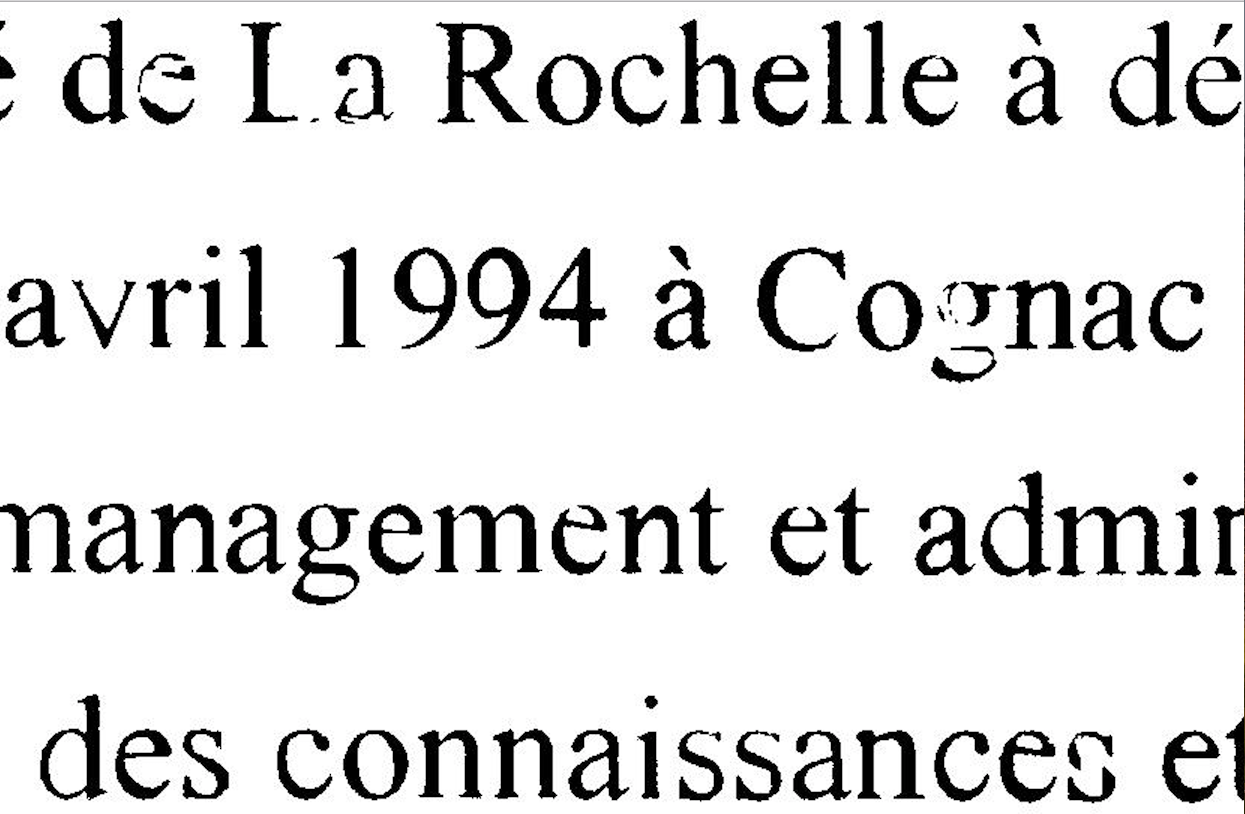
\includegraphics[trim = 0cm 0cm 0cm 0cm, clip,scale=0.066]{./images/Fuzzy_Cluster_Defaults.png}}
		\caption{}
		\label{image_text_1}
	\end{subfigure}       
	\caption[startProcess]{Various preprocessing steps: (a) Original gray image (b) Gradient image obtained by \cite{Dollar2013} (c) Anisotropic filtered image (d) Edge detected by canny  (e) Dilated images after canny edge detection (f) Hole filled image after dilation (g) Selected textual regions $\mathcal{T}(x,y)$ (h) Only sure text pixels after clustering  (i) Sure and confused pixels after clustering (j) Existing issue of character deformation after clustering (sure text pixels only).  }
	\label{allPreprocessing}
\end{figure*}

\begin{table}[h!]
	\centering
	\begin{tabular}{||p{1.5cm} p{1.8cm} || p{1.5cm} p{1.8cm}||} 
		\hline
		\centering
		\textbf{Method Name} & \centering \textbf{Time Required} & \centering \textbf{Method Name} & \centering \textbf{Time Required} \tabularnewline
		\hline\hline
		\centering
		FCM\_S1 & \centering 232.15 & \centering FGFCM\_S2 &  \centering 2.23 \tabularnewline
		\centering
		FCM\_S2 & \centering 201.14 & \centering ENFSCM &  \centering 0.74 \tabularnewline
		\centering
		FCM\_M1 & \centering 3.07 & \centering FLICM &  \centering 662.25 \tabularnewline
		\centering
		FGFCM & \centering 2.15 & \centering FRFCM &  \centering 0.27 \tabularnewline
		\centering
		FGFCM\_S1 & \centering 1.79 &  &  \\  
		\hline
	\end{tabular}
	\caption{Time required (in seconds) by the different clustering algorithm on a cropped diploma image.}
	\label{table:clusteringTime}
\end{table}

\subsection{Fuzzy C-Means (FRFCM) Clustering Algorithm}
\label{FRFCM}
Following to the aforementioned state of the art on FCM clustering mentioned in Section \ref{related_work}, Lei and Jia et al.\cite{Lei2017} proposed  FRFCM algorithm with a low computational cost which can achieve good segmentation results for various types of images and can also achieve high segmentation precision. It employs morphological reconstruction (MR) to smooth the images in order to improve noise immunity and image detail preservation. Results obtained by various aforementioned clustering techniques on a small cropped image of $822 \times 674$ are shown in Table \ref{table:clusteringTime}. It can be seen that FRFCM has an impressive computational time.

Therefore, FRFCM is faster than other aforementioned improved FCM algorithms. By setting the number of clusters to $3$ (sure text pixels, confused text pixels and background pixels), we apply FRFCM clustering on $\mathcal{T}(x,y)$ (i.e. on the image shown in Fig.\ref{image_text_7} ), which gives a clustered image (see Fig. \ref{image_text_9}). The two deeper intensities are visible in Fig. \ref{image_text_9} except white, which represent the background. Among these two deeper intensities, the darker one represents the intensities of \textit{sure text pixels} (the image formed by only these pixels are shown in Fig. \ref{image_text_8}) and the other ones represent \textit{confused pixels}. The following mentioned techniques are applied to qualify these pixels as texts or background.  

Some character shapes are deformed due to clustering (see Fig. \ref{image_text_1}) but this problem mainly comes from the gradient image formation followed by the Canny edge detection. Due to the low contrast between the background and foreground at these specific regions of the image, the gradient image fails to clearly signify text regions followed by the failure of Canny's edge detection. 
This is shown in Fig.  \ref{image_text_10}  (top left: zoomed portion of dilated image after canny, top right: hole filled image, bottom left: textual region separation bottom, right: clustered image). Note that even before performing the dilation operation on the Canny image, some portions of the image were already missing.  The following technique is applied to recover the missing portions and to reconstruct the image.
%		\begin{figure*}[h]
%		\centering
%		\begin{subfigure}[b]{0.09\textwidth}
%			\centering\fbox{
\includegraphics[trim = 0cm 0cm 0cm 0cm, clip,scale=0.07]{./images/AllClustering/test_Clustering_2.png}}
%			\caption{}
%			\label{clustering_0}
%		\end{subfigure}%
%		~%add desired spacing between images, e. g. ~, \quad, \qquad etc.
%		\begin{subfigure}[b]{0.09\textwidth}
%			\centering	\fbox{
\includegraphics[trim = 4.4cm 4.6cm 4.4cm 2.4cm, clip,scale=0.08]{./images/AllClustering/FCM_s1.png}}
%			\caption{}
%			\label{clustering_1}
%		\end{subfigure}	
%		~%add desired spacing between images, e. g. ~, \quad, \qquad etc.		 			        
%		\begin{subfigure}[b]{0.09\textwidth}
%			\centering \fbox{
\includegraphics[trim = 4.4cm 4.6cm 4.4cm 2.4cm, clip,scale=0.08]{./images/AllClustering/FCM_s2.png}}
%			\caption{}
%			\label{clustering_2}
%		\end{subfigure}%
%		~%add desired spacing between images, e. g. ~, \quad, \qquad etc.		 			        
%		\begin{subfigure}[b]{0.09\textwidth}
%			\centering \fbox{
\includegraphics[trim = 4.4cm 4.6cm 4.4cm 2.4cm, clip,scale=0.08]{./images/AllClustering/FCM_m1.png}}
%			\caption{}
%			\label{clustering_3}
%		\end{subfigure}%
%		~%add desired spacing between images, e. g. ~, \quad, \qquad etc.		
%		\begin{subfigure}[b]{0.09\textwidth}
%			\centering \fbox{
\includegraphics[trim = 4.4cm 4.6cm 4.4cm 2.4cm, clip,scale=0.08]{./images/AllClustering/Fgfcm.png}}
%			\caption{}
%			\label{clustering_4}
%		\end{subfigure}
%		~%add desired spacing between images, e. g. ~, \quad, \qquad etc.
%		\begin{subfigure}[b]{0.09\textwidth}
%			\centering \fbox{
\includegraphics[trim = 4.4cm 4.6cm 4.4cm 2.4cm, clip,scale=0.08]{./images/AllClustering/Fgfcm_S1.png}}
%			\caption{}
%			\label{clustering_5}
%		\end{subfigure}	
%		~%add desired spacing between images, e. g. ~, \quad, \qquad etc.	
%		\begin{subfigure}[b]{0.09\textwidth}
%			\centering \fbox{
\includegraphics[trim = 4.4cm 4.6cm 4.4cm 2.4cm, clip,scale=0.08]{./images/AllClustering/Fgfcm_S2.png}}
%			\caption{}
%			\label{clustering_6}
%		\end{subfigure}	
%		~%add desired spacing between images, e. g. ~, \quad, \qquad etc.
%		\begin{subfigure}[b]{0.09\textwidth}
%			\centering \fbox{
\includegraphics[trim = 4.4cm 4.6cm 4.4cm 2.4cm, clip,scale=0.08]{./images/AllClustering/FLICM.png}}
%			\caption{}
%			\label{clustering_7}
%		\end{subfigure}		
%		~%add desired spacing between images, e. g. ~, \quad, \qquad etc.
%		\begin{subfigure}[b]{0.09\textwidth}
%			\centering \fbox{
\includegraphics[trim = 4.4cm 4.6cm 4.4cm 2.4cm, clip,scale=0.08]{./images/AllClustering/EnFCM.png}}
%			\caption{}
%			\label{clustering_8}
%		\end{subfigure}		
%		~%add desired spacing between images, e. g. ~, \quad, \qquad etc.
%		\begin{subfigure}[b]{0.09\textwidth}
%			\centering \fbox{
\includegraphics[trim = 4.4cm 4.6cm 4.4cm 2.4cm, clip,scale=0.08]{./images/AllClustering/FRFCM.png}}
%			\caption{}
%			\label{clustering_9}
%		\end{subfigure}	       
%		\caption[allClustering]{Results obtained by different clustering algorithm on a cropped diploma image. (a): The background separated cropped image, (b)Result by FCM\_S1 (\textit{232.15 sec.}) (c) Result by FCM\_S2 (\textit{201.14 sec.}) (d) Result by FCM\_M1 (\textit{3.07 sec.}) (e) Result by FGFCM (\textit{2.15 sec.}) (f) Result by FGFCM\_S1 (\textit{1.79 sec.}) (g) Result by FGFCM\_S2 (\textit{2.23 sec.}) (h) Result by ENFSCM(\textit{0.74 sec.}) (i) Result by FLICM (\textit{662.25 sec.}) (j) Result by \textbf{FRFCM}: The chosen algorithm for our problem (\textit{0.27 sec.})}
%		\label{fig:clusteringResult}
%	\end{figure*}
\subsection{Savoula Binarization} \label{savoulaBin} We apply Savoula binarization \cite{Sauvola2000} on the original image at this step of the algorithm (see Fig. \ref{image_text_11}). The following thresholding formula is used:
\begin{equation}
\begin{split}
\mathcal{S} = m(1-k(1-\frac{\sigma}{R}))
\end{split} 
\label{savoulaThresh}
\end{equation}
where $ k$ is equal to $0.2$ and $R = 125$ is a gray-level range value and $m$, $\sigma$ represents the mean and standard deviation of image window respectively. 

\subsection {Basic and Fast Text Line Segmentation } \label{textlineSeg} Text lines are roughly segmented based on a horizontal projection of the binarized image, obtained by the FRFCM clustering (the sure text pixels). After obtaining the heights of each text line, a simple but efficient approach to calculate the average of these values are described in Algorithm \ref*{algo:averageCalc}. This technique\footnote{Please note that, may be for our case of diploma images, as there are not many text lines, this approach may not show high difference in results, compared to classical averaging but when there are more data, this technique shows better performance.} is helpful for removing outliers from the set of values which helps to calculate a better average value. The values are stored in $Arr[items]$ and the intelligent average is obtained in the variable $AvgVal$. \footnote{We use $hist$ function of Matlab toolbox to calculate histogram of values, divided into 10 bins.} 
%	The horizontal projection basically counts number of pixels in each row. 	 
% \mathcal{A} = Average {\mathcal{H}_t} if  \mathcal{H}_t} > 0
%	\[
%	\mathcal{H}^t = 
%	\begin{cases}
%	k & \text{if } \xi >0 \\
%	0,              & \text{otherwise}
%	\end{cases}
%	1 \leq t \leq M
%	\]
%	Where $\mathcal{H}$ is an array which stores the number of foreground pixels at each row of the image and $M$ is the total number of rows. After that the horizontal projection array is smoothed by using the technique mentioned in Algorithm \ref{algo:Smoothing}. It simply replaces the each cell value with the average value (line $7$ in Algorithm \ref{algo:Smoothing}) by sliding a smoothing mask of size $7$ (empirically set) over each cell (line $3$ in Algorithm \ref{algo:Smoothing}), by putting the mask center on each cell (line $5$ in Algorithm \ref{algo:Smoothing}). 
%	\begin{algorithm}[bht!] 
%		\LinesNumbered
%		\DontPrintSemicolon
%		\KwIn{$\mathcal{H}^{t}, M$}
%		\KwOut{$\mathcal{H}_{smooth}^{t}$}
%		$maskSize \gets 7$ \tcp*{smoothing mask size}
%		\tcc{\textit{floor} func rounds-up value towards ($-\infty$)}
%		$smoothWin \gets floor(maskSize /2)$ \; 
%		\For{$i \gets (smoothWin+1)$ \textbf{to} $(M - smoothWin)$} {
%			$getSum \gets 0$ \; 
%			\For{$j \gets (-smoothWin)$ \textbf{to} $smoothWin$} {
%					$getSum \gets getSum + (double) \mathcal{H}{(i+j,1)}$ \; 
%			}
%			\tcc{\textit{round} func rounds-up the value}
%			\vspace{-0mm}
%			$\mathcal{H}_{smoothed}(i,1) \gets (round)(getSum/maskSize)$ 
%		}
%		\caption{{\sc Smoothing of $\mathcal{H}$ }}
%		\label{algo:Smoothing}
%	\end{algorithm}   
% 	After obtaining the smoothed horizontal projection array ($\mathcal{H}_{smooth}^{t}$), we calculate the average (see $Equation$ \refeq{lineSeg2}) of these values. \footnote{average is calculated over those rows only, which has at-least one foreground pixel.} 
% 	\begin{equation}
% 		\begin{split}
% 			\mathcal{A} = Average \{\mathcal{H}^{t}\} ; \hspace{2mm} if \hspace{2mm} \mathcal{H}^{t} > 0
% 		\end{split} 
%		 \label{lineSeg2}
% 	\end{equation}
% 	Now using this smoothed horizontal projection array ($\mathcal{H}_{smooth}^{t}$) and  number of average foreground pixels $\mathcal{A} $, the segmentation of text line is performed by using Algorithm \ref{algo:lineSegment}.\footnote {It is assumed that text (foreground) is black and background is white. It is also assumed that text starts and ends in the page, having some top and bottom border.}  
%  	For considering any image row as text line or not, we set a threshold ($lnThresh$) of $20\%$ of $\mathcal{A}$.  
% 	Now to get the start of a text line, the idea is that the number of foreground pixels should be more this threshold $lnThresh$ and should also maintain a continuity (line $6-19$ in Algorithm \ref{algo:lineSegment}) of $7$ pixels (empirically set, named as $contThresh$). To detect end of any text line, whose start is already obtained, we
% 	initiate looping from start line (line $13$ in Algorithm \ref{algo:lineSegment}) and try to get the row where the current row has number fore-ground pixel is greater than threshold ($lnThresh$) and the next row has number of fore-ground pixels less than threshold ($lnThresh$) (line $14$ in Algorithm \ref{algo:lineSegment}). If this end line condition is satisfied then look for the continuity (number of fore-ground pixels should be continuously (line $16-18$ in Algorithm \ref{algo:lineSegment}) less than threshold ($lnThresh$) ). So, by using the technique mentioned in Algorithm \ref{algo:lineSegment}, we obtain the start and end line indexes along with the height of each line in an array ($txtLnEntri$). 

% 	\begin{algorithm}%[bht!] 
% 	 %	\begin{minipage}{0.56\textwidth}	
%	 		\LinesNumbered
%	 		\DontPrintSemicolon
%	 		\KwIn{$\mathcal{H}_{smooth}^{t}, M,  \mathcal{A}  $}
%	 		\KwOut{$txtLnEntri$ (storing start and end indexes of each text lines)}
%	 		\tcc{no. of foreground pixels threshold }
%	 		\vspace{-0mm}
%	 		$ lnThresh \gets (round)(\mathcal{A} \% 20) $ \;
%	 		\tcc{Counting number of lines }
%	 		\vspace{-0mm}
%	 		$ p\gets 1$; $contThresh = 7$; $lnImg \gets 1 $  \;
%	 		\While{$ p \leq (M - 1) $} {
%	 			\tcc{If no. of foreground pixels $>$ threshold }
%	 			\vspace{-4mm}
%	 			\uIf{$ \mathcal{H}_{smoothed} (p,1) > lnThresh $}{
%			 			$ cnt \gets 0 $ \; 
%			 			\tcc{Check for continuity of rows, having no. of foreground pixels $>$ threshold }
%			 			\vspace{-4mm}
%			 			\For{$ ut \gets 1$ \textbf{to} $(contThresh - 1) $} {
%			 					\uIf{$ \mathcal{H}_{smoothed} ((p + ut),1) \ge lnThresh $}{
%			 						$ cnt = cnt +1 $\; 
%			 					}
%		 				}
%	 					\tcc{Check if continuity is equal to \textit{contThresh} }
%	 					\vspace{-0mm}
%		 				\uIf{$ cnt == (contThresh-1) $}{
%				       $ startLnFlg = true $; $ startLn = p $\;
%				       \tcc{Store \textit{startLn} index in an array }
%				       \vspace{-4mm}
%				       $ txtLnEntri(lnImg,1) = startLn $\;
%		 				}	
% 				}
% 				\tcc{If we have already got the start line then look for end line }
% 				\vspace{-0mm}
%		 		\uIf{$ startLnFlg = true) $}{ 	
%		 				\tcc{Loop from start line until obtaining the end line }
%		 				\vspace{-0mm}
%				 		\For{$ iko \gets startLn$ \textbf{to} $M - 1 $} {
%				 			\tcc{Check for the condition where current row has no. foreground pixels more than \textit{lnThresh} but next row hasn't }
%				 			\vspace{-0mm}
%				 				 \uIf{$ ((\mathcal{H}_{smooth}(iko,1) \geq lnThresh) \&
%				 				 		 (\mathcal{H}_{smooth}(iko+1,1) \leq lnThresh) ) $}{
%				 						$ cnt = 0 $\;
%				 						\tcc{Check continuity of rows, having no. of foreground pixels less than threshold }
%				 						\vspace{-0mm}
%				 						\For{$ ut \gets 1 $ \textbf{to} $ (contThresh-1) $} {
%				 							 \uIf{$ (\mathcal{H}_{smooth}((iko+ut),1) < lnThresh) $}{
%				 									$ cnt = cnt +1 $\;
%				 								}
%								 		}
%							 		\tcc{Check if continuity is equal to \textit{contThresh} }
%							 		\vspace{-0mm}
%				 					\uIf{$ (cnt == (contThresh-1)) $}{
%				 							$ endLn = iko $\;
%				 							\tcc{Store \textit{endLn} index}
%				 							\vspace{-0mm}
%				 							$ txtLnEntri(lnImg,2) = endLn $\;
%				 							\tcc{Store height of detected line }
%				 							\vspace{-0mm}
%				 							$ txtLnEntri(lnImg,3) = endLn - startLn$ \;
%				 							\tcc{reset the flag and forward $p$ for above $while$ loop }
%				 							\vspace{-0mm}
%				 							$ startLnFlg = false $; $ p = endLn $\; 
%				 							$ lnImg ++ $\;
%				 							$ break $\;
%				 					}
%				 				}
%				 		}
%		 		}
%		 		$p = p +1$\; 
%	 	}
% 		\caption{{\sc Simple and Fast Text Line Segmentation }}
% 		\label{algo:lineSegment}
% 	%	\end{minipage}
% 	\end{algorithm}  

\begin{algorithm}
	%\DontPrintSemicolon % Some LaTeX compilers require you to use \dontprintsemicolon    instead
	\KwIn{Arr[items]}
	\KwOut{AvgVal}
	Divide the elements in $10$ equal spaced bins (we use $hist$ function of Matlab)\\
	From the bin centers of each bins, get the  lower and upper limit of each bin\\
	Sort the bins based on number of elements exists in each bin \\
	Only consider top two bins\\
	Choose those values which belongs to these two top bins (using upper and lower limits of each bin). Let's call them refined values (denoted as $Refined[items]$) \\
	Calculate mean $(\mathbf{M})$ and standard deviation ($\mathbf{S}$) from these refined values  \\
	Now again obtain the re-refined values by verifying if it belongs to : $(\mathbf{M} - \mathbf{S}) \leq Refined[items] \leq (\mathbf{M} - \mathbf{S})$\\
	Finally calculate mean from these re-refined values\\
	\caption{INTELLIGENT AVERAGING}
	\label{algo:averageCalc}
\end{algorithm}

\subsection {Window Based Image Binarization } \label{windowBasedBin} We apply a fast window based binarization technique on the original gray image. This technique is inspired by the method in \cite{Bataineh2011}. From the previous step of text line segmentation, we get the very first ($textStart$) and the last image row ($textEnd$), which contains text. As we already have the average height of text lines ($AvgVal$) so by using this information, we divide the image of considerable region (region between $textStart$ and $textEnd$) into equal size horizontal stripes. Now each horizontal stripes is divided into $20$ equal parts\footnote{Considering the resolution of image, we choose this value as $20$. The objective is to get small textual region for local binarization. We have not properly tested this chosen value so the performance can be slightly improved by the proper choice of this value by evaluating on some test dataset.} and each of these parts called (\textit{"window"}) on which the binarization is performed by using the following Equation \ref {dynamicBin_1} and \ref{dynamicBin_2}.
\begin{equation}
\begin{split}
\sigma_{adaptive} = [\frac{\sigma_{W} - \sigma_{min}}{\sigma_{max} - \sigma_{min}}] \times max_{Intensity}
\end{split} 
\label{dynamicBin_1}
\end{equation}
\begin{equation}
\begin{split}
\mathcal{T}_{W} = \mathcal{M}_{W} - \frac{\mathcal{M}_{W} \times \sigma_{W}}{(\mathcal{M}_{W} + \sigma_{W}) (\sigma_{adaptive} + \sigma_{W})}
\end{split} 
\label{dynamicBin_2}
\end{equation}
where $\sigma_{adaptive}$ is the gray level value of the adaptive standard deviation of the window. $\sigma_{W}$ is the standard deviation of the window, $\sigma_{min}$ and $\sigma_{max}$ are the minimum  and maximum standard deviation of all the windows ($20$ here), $max_{Intensity}$ is the maximum intensity value of the horizontal stripe, $\mathcal{M}_{W}$ is the mean value of the pixel intensities of the window and $\mathcal{T}_{W}$ is the threshold of the window.  
%	\begin{equation} 
%	 	\label{dynamicBin_3}
%	 	WinImg^{binary}(x,y) = 
%	 	\begin{cases}
%		 	0 & \text{if } WinImg(x,y) < \mathcal{T}_{W} \\
%		 	255,  & WinImg(x,y) \geq \mathcal{T}_{W} 
%	 	\end{cases}
% 	\end{equation}	
The obtained binarized image is denoted by $WinImg^{binary}(x,y)$ (see Fig. \ref{image_text_12}). It can be seen that although the simple Savoula binarization has comparatively performed well but it fails to remove the centered decorated background (called \textit{"couronne"} in French) whereas the binarized image from window Based Image Binarization is prominently keeping most of the background decorated portions. So, none of these can be directly used for our case.  

\begin{algorithm}[bht!] 
	%	\begin{minipage}{0.56\textwidth}
	\LinesNumbered
	\DontPrintSemicolon
	\KwIn{$\gamma$, $\beta$, $MRows$, $NCols$}
	\KwOut{$\mathcal{H}_{smooth}$}
	$maskSz \gets 5$ \Comment{\textit{mask size for reconstruction}} \; 
	$winSz = maskSz/2$\;
	$combi\_Imag \gets \gamma$ \; 
	$sum \gets 0$ \; 
	\For{$iR \gets 0$ \textbf{to} $(M-1)$} {
		\For{$jC \gets 0$ \textbf{to} $(N-1)$} {
			\tcc{Verifying the confused pixels in clustered image}
			\vspace{-0mm}
			\uIf{$(\beta(iR, jC) \neq 0)$ \& $(\beta(iR, jC) \neq 255)$}{
				\tcc{check if this pixel is text in both in savoula and windowed binary image}
				\vspace{-0mm}
				\uIf{$(\Upsilon(iR, jC) = 0)$ \& $(\chi(iR, jC) = 0)$}{
					$ sCnt \gets 0$; $x1 \gets 0$; $y1 \gets 0$\;
					\For{$k \gets -winSz$ \textbf{to} $winSz$} {
						\For{$c \gets -winSz$ \textbf{to} $winSz$} {
							%											 \tcc{Avoid center pixel}
							%											\uIf{$(k \neq 0)$ \& $(j \neq 0)$}{
							%												$ x1 = Handle\_Bound(NCols, jC-j)$\;  
							%												$ y1 = Handle\_Bound(NRows, iR-k)$\;  
							\tcc{ counting the number of strong pixels at the surrounding}
							\uIf{$ (\Upsilon(y1, x1) == 0) \, \& \, (\chi(y1, x1) == 0)$}{ 
								$sCnt++$
							}
							%											}
						}
					}
					%					\tcc{ if number of strong pixels is more that 40\% of total pixels in the neighbourghood}
					%							\tcc{-1 to avoid counting the center pixel}	
					\uIf{$(sCnt \ge ((0.2 \times winSz^2)-1 )$}{
						$combi\_Imag(iR, jC) = 0$\;
						$\beta(iR, jC) = 0$\;
					}
				}
			}
		}
	}
	\caption{\sc Character Reconstruction}
	\label{algo:pixelReconstruc}
	**$\gamma$ (sure text pixels), $\beta$ (sure and confused text pixels), $MRows$ (Total number of image rows), $NCols$ (Total number of image columns).
	% \end{minipage}
\end{algorithm} 

\subsection {Reconstruction of Deformed Characters} \label{reconstruction}
We propose a technique for the reconstruction of deformed characters with the help of Savoula and Window based binary image. This reconstruction is required as the shape of the characters should remain intact for proper decoding of the secret number, as mentioned in introduction (see section \ref{intro}). The obvious text pixels (sure text pixels), obtained from the fuzzy clustering are copied into a new image (called $\mathcal{K}(x,y)$). Now, for each confused pixel (line $7$ in Algorithm \ref{algo:pixelReconstruc}) in the fuzzy clustered image, we check first if the same pixel is a foreground pixel in Savoula image ($\Upsilon$) and  also in window based binary image $(\chi)$. If they are foreground pixels (line 8 in Algorithm \ref{algo:pixelReconstruc}) then we traverse at the neighborhood of this pixel with the window size of $winSz \times winSz$ and count the number of such pixels which are foreground both in $\Upsilon(x, y)$ and $\chi(x, y)$.
If this number exceeds $20\%$ of the window size ($winSz \times winSz$) (line $17$ in Algorithm \ref{algo:pixelReconstruc}), then we mark this pixel as text pixel otherwise it is marked as background pixel. The value of $winSz$ is taken as $(\emph{\text{stroke width} / 2})$. The $\emph{\text{stroke width}}$ is calculated by using the approach, mentioned in \cite{BolanSu2013}.  
%The value of $winSz$ is taken as $\text{stroke width} / 2$. The $\text{stroke width}$ is calculated by using the approach, mentioned in \cite{BolanSu2013}. 
%The underlying idea is to compute an adaptive local contrast image based on the neighboring maximum and minimum intensity value of each pixel to properly detect the stroke edge pixels of the document text.
The recovered and background separated image is shown in Fig. \ref{image_text_14} and one the zoomed portion is shown in Fig. \ref{image_text_13}). 
%Then edges are detected based on the combination of Canny's edge detector and Otsu's thresholding technique. After that the stroke width ($W_{stroke}$) is calculated by traversing each image row and by finding the distance between two edge pixels (whose binary image value is $1$ and has higher gray level intensity than the next pixel, having binary value $0$ and has lower intensity) and then averaging such distances all together.
\begin{figure}[bht!]
%	\begin{minipage}{0.5\textwidth}
		\centering
		\begin{subfigure}[b]{0.49\textwidth}
			\centering\fbox{
\includegraphics[trim = 2.9cm 19.5cm 3.1cm 2.9cm, clip,scale=0.42]{./images/Find_Prob/error_reason.pdf}}
			\caption{}
			\label{image_text_10}
		\end{subfigure}	
		\begin{subfigure}[b]{0.49\textwidth}
			\centering \fbox{
\includegraphics[trim = 0cm 0cm 0cm 0cm, clip,scale=0.018]{./images/Savoula_Binary_Image.jpg}}
			\caption{}
			\label{image_text_11}
		\end{subfigure}
		\newline	
		\begin{subfigure}[b]{0.32\textwidth}
			\centering \fbox{\includegraphics[trim = 0cm 0cm 0cm 0cm, clip,scale=0.016]{./images/Mixed_Binary_Image.jpg}}
			\centering\caption{}
			\label{image_text_12}
		\end{subfigure}			
		\begin{subfigure}[b]{0.32\textwidth}
			\centering \fbox{
\includegraphics[trim = 0cm 0cm 0cm 0cm, clip,scale=0.016]{./images/CombinedOpen_Binary_Image.jpg}}
			\caption{}
			\label{image_text_14}
		\end{subfigure}	
		\begin{subfigure}[b]{0.32\textwidth}
			\centering \fbox{
\includegraphics[trim = 0cm 0cm 0cm 0cm, clip,scale=0.090]{./images/CombinedOpenBin_correction.png}}
			\caption{}
			\label{image_text_13}
		\end{subfigure} 
		\caption[endProcess]{(a): Reasons of character deformation (b) Binary image by Savoula technique (c) Binary image by Dynamic window based technique (d) The text separated image after reconstruction (e) Zoomed portion after image reconstruction }
		\label{fig:finalresul}
%	\end{minipage}
\end{figure}
% \begin{algorithm}
% 	\caption{HANDLE IMAGE BOUNDARY}
% 	\begin{algorithmic}[1]
% 		\Procedure{Handle\_Bound}{$P, x$}
% 		
%		\If{$x < 0$}{
%			\hspace{5mm} $return$ $(-x-1)$\; 
%		}
%		\If{$x \geq P$}{
%			\hspace{5mm} $return$ $((2*P)-x-1)$\; 
%		}
%		$return $ $x$\;
% 		\EndProcedure
% 	\end{algorithmic}
% \end{algorithm}

% 	\begin{algorithm}[bht!] 
%	\LinesNumbered
%	\DontPrintSemicolon
%	\KwIn{$P$ (maximum limit), $x$ (index)}
%	\KwOut{$x$ (boundary conditioned index)}
%		\uIf{$x < 0$}{
%			$return$ $(-x-1)$\; 
%		}
%		\uIf{$x \geq P$}{
%			$return$ $((2*P)-x-1)$\; 
%		}
%	$return $ $x$\;
%	\caption{{\sc Handle\_Boundary() }}
%	\label{algo:BoundaryCond}
%\end{algorithm}  
\section {Results and Discussion }
\label{results}
In this section, we will mention and discuss the obtained results on dataset of university diplomas.  
\subsection{Dataset}
To evaluate the proposed algorithm, we have created the French university diploma dataset described in the following.
\subsubsection{Diploma Data set : }  
Total $40$ images were scanned in colored  and gray level (mentioned as Dip\_Col and Dip\_Gray in Table. \ref{tab:allResultStats}) by \textit{"Fujitsu"} scanner in $300$ (20 images) and $600$ (20 images) DPI (of size is $7000 \times 5000$ pixels approx.). 
%Color images are manually converted to gray scale before manually erasing confidential information from the diplomas. 
\paragraph{Ground Truth Preparation : } 
Due to no prior availability of dataset, we have created a dataset and corresponding GT. Due to high image size, it is cumbersome to create the GT manually. So, we adapted a semi manual approach by manually selecting the range of the gray level threshold for foreground / text pixels\footnote{Data and available at : \url{https://github.com/tanmayGIT/University_Diploma_BackGd_Removal.git}\label{gitlink}}. Then the obtained images are manually corrected by GIMP software.\footnote{ These documents are real \textit{University of La Rochelle, France} diplomas of students. We avoid to generate fake diplomas as it is forbidden by the law. For the privacy purpose, the confidential information e.g. name, date of birth, unique number of diploma etc. are manually removed from the gray image (for color images, it was first converted into gray)} 
%\subsubsection{DIBCO Data set :} 
%Although the proposed algorithm is designed for background removal of French university diplomas but as this specific topic has some resemblance with document image binarization, we have also tested the efficiency of the proposed algorithm on DIBCO public data sets from previous document image binarization competitions: H-DIBCO'12, DIBCO'13, H-DIBCO'14, H-DIBCO'16 and DIBCO'17. 
%The DIBCO'13 and DIBCO'17 contains both handwritten and machine-printed images while the other ones only contain handwritten images (for more details, see in \cite{Pratikakis2018}).  
%}
\begin{table}[bht!]
	\centering
	%\begin{minipage}[b]{0.5\textwidth}
	\begin{threeparttable}
		\centering\small
		\caption{Result on University Diploma Dataset\label{tab:allResultStats}. The best results of each metric are highlighted in bold.}
		\centering
		\begin{tabular}{ P{1.4cm} P{1.2cm} P{1.8cm} P{1.8cm} P{1.2cm} P{1.4cm} }
			\toprule
			\centering
			{Dataset} &{No. of Images} &\centering{Method Name}  & \centering{F-Measure (\%)($\uparrow$)} & {PSNR} ($\uparrow$)& {DRD}($\downarrow$) \\ \midrule \midrule
			\centering
			{300\_Col}  &  10& \cellcolor{gray}{Proposed} & \cellcolor{gray}89.89 & \cellcolor{gray}20.90 & \cellcolor{gray}5.56 
			\\ & & Niblack & 10.26 & 2.03 & 501.80 
			\\ & & Savoula & 87.70 & 19.98 & 7.90 
			\\ & & Wolf-Jolin & 83.90 & 18.60 & 11.22 \\ 
			& & Bataineh \cite{Bataineh2011} & 68.88 & 14.80 & 30.24 \\
			& & Gatos \cite{Gatos2006} & 84.74 & 18.80 & 10.75 \\
			& & Mondal \cite{Mondal2019} & 84.40 & 19.05 & 9.39 \\
			& & Jia \cite{Jia2018} (\textcolor{blue}{for 10 images}) & 71.88 & 15.48 & 25.84 \\
			\midrule
			\centering
			{300\_Gray}  & 10 &\cellcolor{gray} {Proposed} & \cellcolor{gray} 93.62 & \cellcolor{gray} 22.90 & \cellcolor{gray} 2.99 
			\\ & & Niblack & 10.61 & 1.85 & 486.97 
			\\ & & Savoula & 91.98 & 21.91 & 4.70 
			\\ & & Wolf-Jolin & 89.40 & 20.50 & 6.56 \\ 
			& & Gatos \cite{Gatos2006} & 91.08 & 21.23 & 5.55 \\
			& & Bataineh \cite{Bataineh2011} & 74.59 & 15.78 & 23.54 \\
			& & Mondal \cite{Mondal2019} & 86.88 & 19.89 & 7.19 \\
			& & Jia \cite{Jia2018} (\textcolor{blue}{for 8 images}) & 87.91 & 19.93 & 8.07 \\
			\midrule
			\centering
			{600\_Col}  & 10 & \cellcolor{gray}{Proposed} &\cellcolor{gray}92.05 & \cellcolor{gray}21.91 & \cellcolor{gray}3.59  
			\\ & & Niblack & 10.83 & 2.09 & 446.60 
			\\ & & Savoula & 89.36 & 20.58 & 5.77 
			\\ & & Wolf-Jolin & 85.88 & 19.16 & 8.40 \\ 
			& & Bataineh \cite{Bataineh2011} & 68.96 & 14.71 & 27.59 \\
			& & Gatos \cite{Gatos2006} & 85.36 & 18.91 & 9.07 \\
			& & Mondal \cite{Mondal2019} & 88.48 & 20.48 & 5.86 \\
			& & Jia \cite{Jia2018} (\textcolor{blue}{for 8 images}) & 85.12 & 19.26 & 8.32 \\
			\midrule
			\centering
			{600\_Gray}  & 10 & \cellcolor{gray}{Proposed} &\cellcolor{gray}95.14 &\cellcolor{gray}24.04 &\cellcolor{gray}1.76  
			\\ & & Niblack & 10.96 & 1.90 & 420.37 
			\\ & & Savoula & 92.12 & 21.89 & 4.03 
			\\ & & Wolf-Jolin & 89.63 & 20.50 & 5.59
			\\ & & Bataineh \cite{Bataineh2011} & 74.92 & 15.75 & 20.44 \\ 
			& & Gatos \cite{Gatos2006} & 91.30 & 21.25 & 4.57 \\ 
			& & Mondal \cite{Mondal2019} & 89.33 & 20.76 & 4.94 \\
			& & Jia \cite{Jia2018} (\textcolor{blue}{for 6 images}) & 83.60 & 18.70 & 11.05 \\
			\midrule 
			\midrule
			
			
			%			\centering
			%			\multirow{4}{*}{DIBCO\_12}  &\multirow{4}{*}{14}& Proposed & 67.72 & 15.68 & 8.78 \\\cline{3-6}
			%			&  & Lelore\cite{Pratikakis2018} & \textbf{94.05} & 21.43 & 2.11 \\\cline{3-6}
			%			&  & Su\cite{Pratikakis2018} & 89.76 & 19.55 & 4.19 \\\cline{3-6}
			%			&  & Howe\cite{Pratikakis2018} & 93.73 & \textbf{21.85} & \textbf{2.10} \\ \midrule \midrule
			%			\centering
			%			\centering
			%			\multirow{4}{*}{DIBCO\_13} &\multirow{4}{*}{16}& Proposed & 74.94&16.31 & 6.63  \\\cline{3-6}
			%			&  & Lelore\cite{Pratikakis2018} & 90.78 & 20.54 & 3.59 \\\cline{3-6}
			%			&  & Su\cite{Pratikakis2018} & 87.70 & 19.59 & 4.21 \\\cline{3-6}
			%			&  & Howe\cite{Pratikakis2018} & \textbf{91.34} & \textbf{21.29} & \textbf{3.18} \\ \midrule \midrule
			%			\centering
			%			\multirow{4}{*}{DIBCO\_14} &\multirow{4}{*}{10}& Proposed & 72.28&14.64 & 8.01 \\\cline{3-6} 
			%			&  & Lelore\cite{Pratikakis2018} & 96.14 & 21.88 & 1.25 \\\cline{3-6}
			%			&  & Su\cite{Pratikakis2018} & 94.38 & 20.31 & 1.95 \\\cline{3-6}
			%			&  & Howe\cite{Pratikakis2018} & \textbf{96.49} & \textbf{22.24} & \textbf{1.08} \\ \midrule \midrule
			%			\centering
			%			\multirow{4}{*}{DIBCO\_16}  &\multirow{4}{*}{10}& Proposed & 79.63&17.11 & 5.84 \\\cline{3-6}  
			%			&  & Lelore\cite{Pratikakis2018} & 87.21 & 17.36 & \textbf{5.27} \\\cline{3-6}
			%			&  & Su\cite{Pratikakis2018} & 84.75 & 17.64 & 5.64 \\\cline{3-6}
			%			&  & Howe\cite{Pratikakis2018} & \textbf{87.47} & \textbf{18.05} & 5.35 \\ \midrule \midrule
			%			\centering
			%			\multirow{2}{*}{DIBCO\_17}  &\multirow{2}{*}{20}& Proposed & 73.98 & 14.60 & 7.15\\\cline{3-6}  
			%			&  & Wei \cite{Pratikakis2018} & \textbf{86.49} & \textbf{16.33} & \textbf{6.57} \\\midrule
			%			% 			\\\cline{3-6}
			%			% 			&  & Cunzhao et al.\cite{Pratikakis2018} & 85.34 & 16.25 & 8.18 \\ 
			
			
		\end{tabular}
		\begin{tablenotes}
			\small
			\item * For the comparison purpose, only training free best performing methods are chosen from literature.  
		\end{tablenotes}
	\end{threeparttable}
	%\end{minipage}
\end{table}

%\subsubsection{F-Measure (FM)} 
%\begin{equation}
%FM = \frac{2 \times Recall \times Precision}{Recall + Precision}
%\end{equation}	
%where $Precison  = \frac{TP}{TP+FR}$ and $Recall = \frac{TP}{TP+FN}$. The $TP$, $FP$ and $FN$ denote the true positive, false positive and false negative values. 

	
	
%	\subsubsection{Pseudo Recall (p-Recall) and Pseudo Precision (p-Precision)} The $pRecall$ and $pPrecison$ metrics use distance weights with respect to the contour of the ground-truth (GT) characters. In the case of $p-Recall$, the weights of the GT foreground are normalized  according to the local stroke width. Generally, those  weights are delimited between $[0,1]$.  In the case of  $pPrecision$, the weights are constrained within an area that expands to the GT background taking into account  the  stroke  width of the nearest GT component. Inside this area, the weights are greater than one (generally delimited between $[1,2]$ while outside this area they are equal to one. 
%	It is defined as the percentage of skeletonized ground truth image that is detected from resulted binary image, obtained by the proposed algorithm. 
%	\begin{equation}
%		p\-Recall = \frac{\sum_{x= 1, y = 1}^{x = M, y = N}SG(x,y).B(x,y)}{\sum_{x=1, y=1}^{x = M, y = N}SG()x,y} \times 100 \%
%	\end{equation}

%	\subsubsection{Pseudo F-Measure (p-FM)} 
%	\begin{equation}
%		pFM = \frac{2 \times pRecall \times pPrecision}{Recall + Precision}
%	\end{equation}
%	The $pRecall$ and $pPrecison$ metrics use distance weights with respect to the contour of the ground-truth (GT) characters (see \ref{Pratikakis2018} for details).


%\subsubsection{Peak Signal to Noise Ratio (PSNR)}
%\begin{equation}
%PSNR = 10\log(\frac{C^2}{MSE})
%\end{equation}
%where $MSE = \frac{\sum_{x=1}^{M}\sum_{y=1}^{N} (I_{bin}(x,y)-I'_{bin}(x,y))}{MN}$; $C$ denotes the difference between text and background. The $PSNR$ measures how close two images are (see \cite{Pratikakis2018} for details).  

%\subsubsection{Distance Reciprocal Distortion Metric (DRD)}
%\begin{equation}
%DRD = \frac{\sum_{k}DRD_k}{NUBN}
%\end{equation}
%where $DRD_k$ is the distortion of the $k-th$ flipped pixel and $NUBN$ is the number of non-uniform (not all black or white pixels) $8\times8$ blocks in the GT image. The $DRD$ is used to measure the visual distortion in binary document images (see \cite{Pratikakis2018} for details). 	
\begin{figure}[bht!]
	\centering 			
	\begin{subfigure}[b]{0.32\linewidth}
		\centering \fbox{
\includegraphics[trim = 0cm 0cm 0cm 0cm, clip,scale=0.138]{./images/GT_Problem.png}}
		\caption{}
		\label{image_text_15}
	\end{subfigure}		
	\begin{subfigure}[b]{0.32\linewidth}
		\centering \fbox{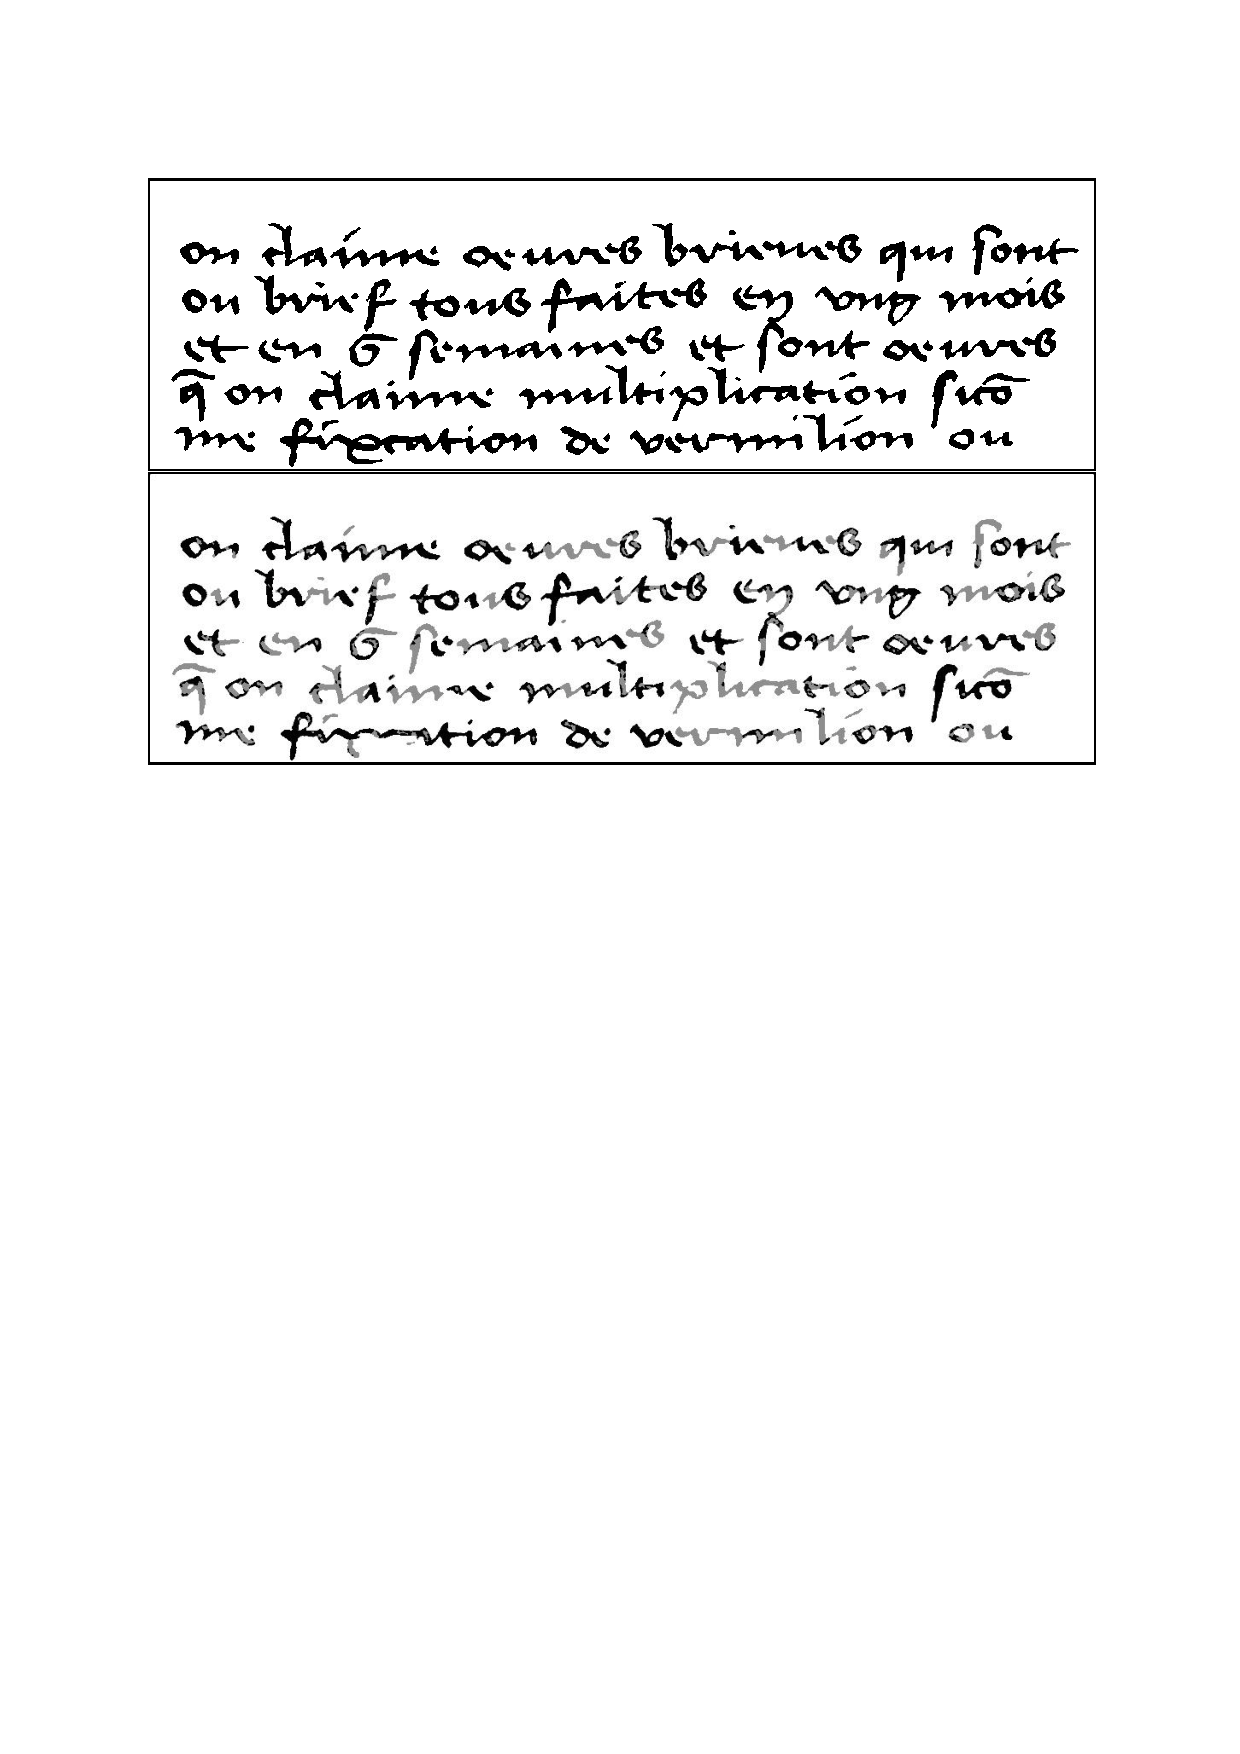
\includegraphics[trim = 7cm 17.5cm 7cm 4cm, clip,scale=0.48]{./images/dibco.pdf}}
		\caption{}
		\label{image_text_16}
	\end{subfigure}	
	\begin{subfigure}[b]{0.32\linewidth}
		\centering \fbox{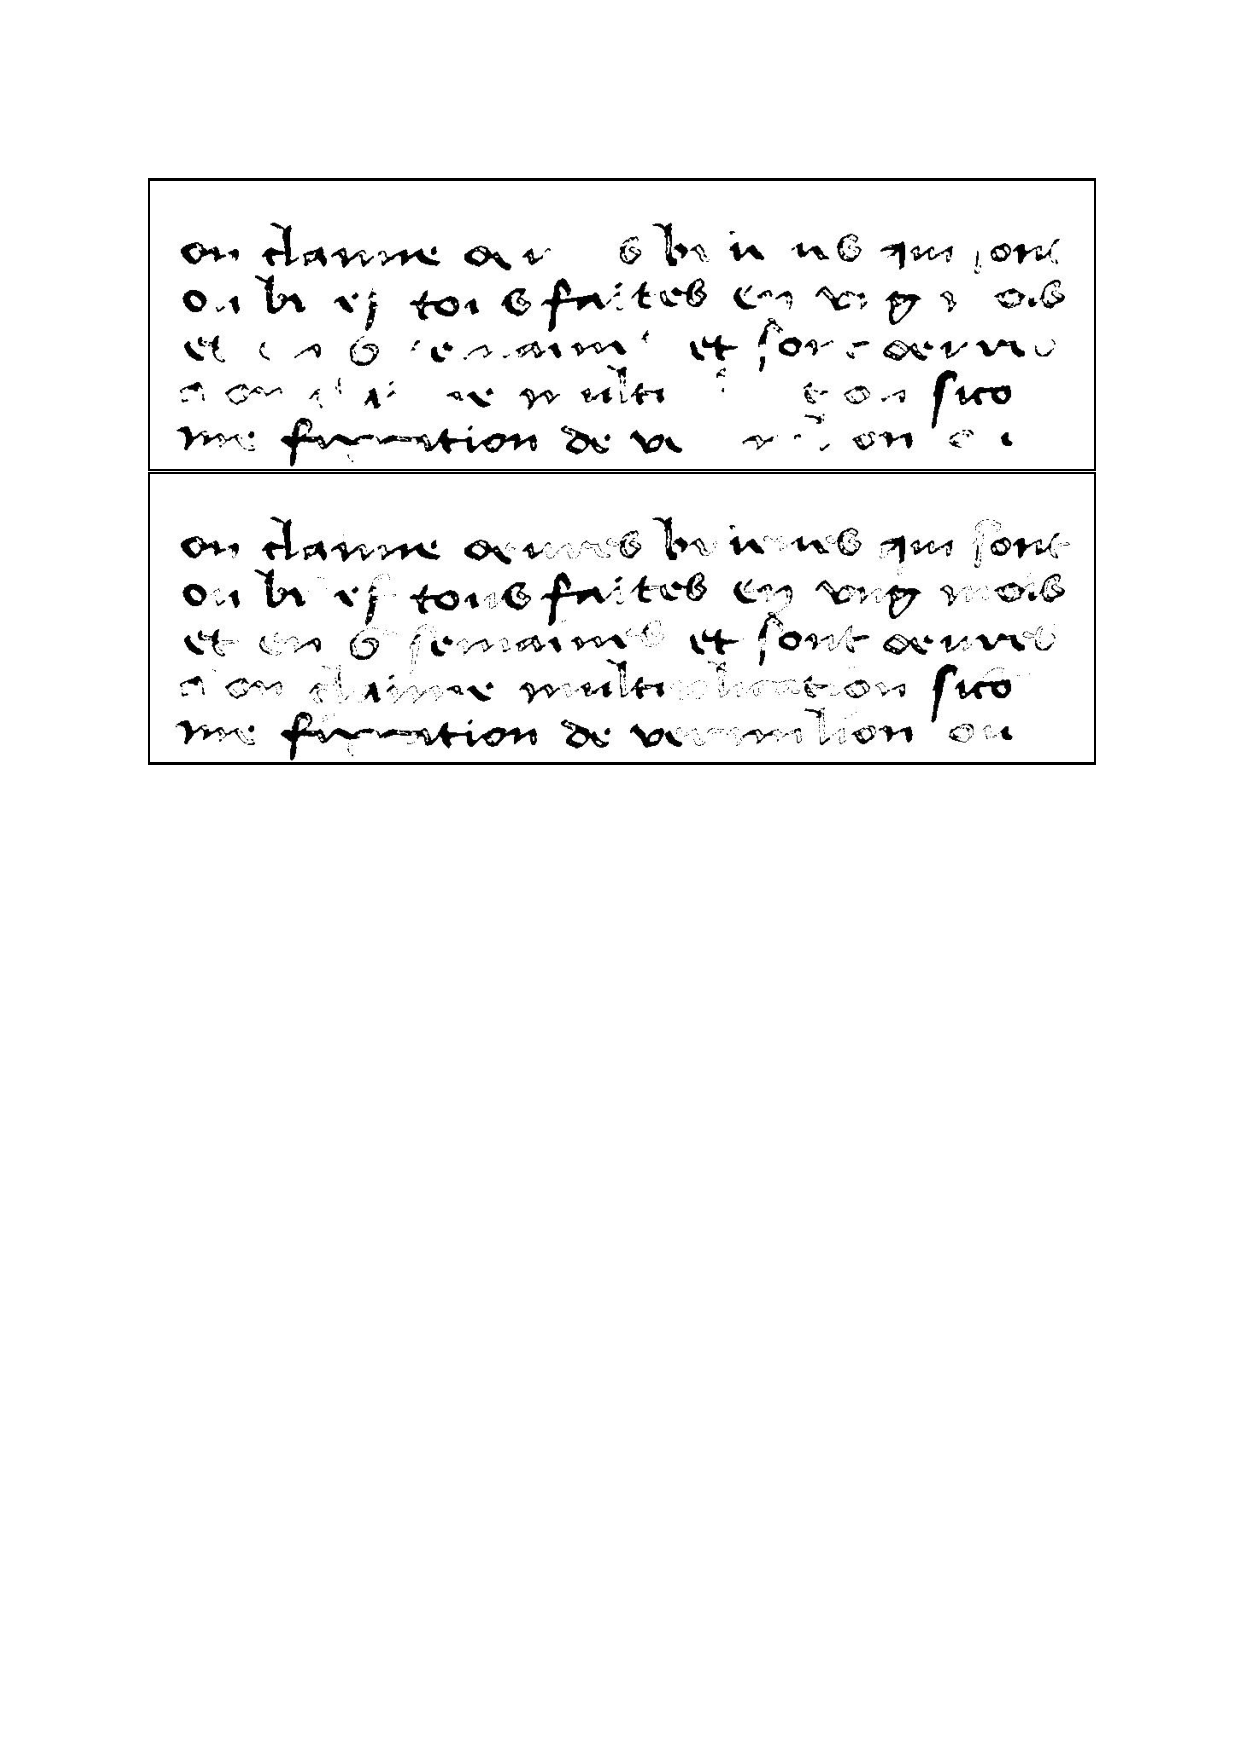
\includegraphics[trim = 7cm 17.5cm 7cm 4cm, clip,scale=0.48]{./images/dibco_res.pdf}}
		\caption{}
		\label{image_text_17}
	\end{subfigure}	       
	\caption[dibcoProbs]{(a): The issues with prepared GT (b) \textit{Top :} One example of GT image from DIBCO dataset; \textit{Bottom :} Clustered image (sure and confused text pixels) (c) \textit{Top :} Only sure text pixels from clustered image \textit{Bottom :} After the image reconstruction}
	\label{fig:dibcoProbsl}
\end{figure}
\subsection{Evaluation Protocol} 
We have used \textit{F-Measure (FM)}, \textit{Peak Signal to Noise Ratio (PSNR)} and Distance Reciprocal Distortion Metric (DRD) as the evaluation metrics (same as DIBCO competition \cite{Pratikakis2018}). 	
It can be seen from Table \ref{tab:allResultStats}, that the performance of our technique is quite promising and achieves an average accuracy (F-Measure) of $93\%$ on four parts of the complete data set. The accuracies could be further improved by a better preparation of the GT (mainly by proper removal of background pixels because our algorithm correctly classifies the background pixels). It can be seen from Fig. \ref{image_text_15} that the GTs are not properly cleaned/corrected, which affected the statistical result. The proposed technique performed better than the classical (e.g. Niblack, Savoula and Wolf-Jolin's \cite{Pratikakis2018}) binarization techniques. However, among these three classical binarization techniques, the Savoula binarization performed comparatively better than others. But as mentioned before that these classical binarization techniques are mainly unable to remove the centered decorated background (i.e. \textit{"couronne"}) (see Savoula binarization result in Fig. \ref{image_text_11} and \ref{image_text_18}).    
\begin{table}[bht!]
	\centering
	\begin{tabular}{||p{2.2cm} p{2.6cm} || p{2.2cm} p{4.4cm}||} 
		\hline
		\centering
		\textbf{Method Name} & \centering \textbf{Time Required} & \centering \textbf{Method Name} & \centering \textbf{Time Required} \tabularnewline
		\hline\hline
		\centering
		Niblack \cite{Pratikakis2018} & \centering 3.03 (\textcolor{blue}{C++}) & \centering Savoula \cite{Pratikakis2018} &  \centering 3.06 (\textcolor{blue}{C++}) \tabularnewline
		\centering
		WolfJolin \cite{Pratikakis2018} & \centering 3.06 (\textcolor{blue}{C++}) & \centering Bataineh \cite{Bataineh2011} &  \centering 1.03 (\textcolor{blue}{C++}) \tabularnewline
		\centering
		Gatos \cite{Gatos2006} & \centering 3.21 (\textcolor{blue}{C++}) & \centering Mondal$^*$ \cite{Mondal2019}  &  \centering 421 + 33.43 + 1031 = 1485.43 (\textcolor{blue}{Matlab and C++}) \tabularnewline
		\centering
		Jia \cite{Jia2018} & \centering 128 (\textcolor{blue}{.exe provided by authors}) & \centering \textbf{Proposed$^{**}$} &  \centering \centering 35.8 + 14 + 5.8 = 55.6 (\textcolor{blue}{Matlab and C++}) \tabularnewline
		\hline
	\end{tabular}
	*Mondal et.al : Background estimation (421 sec. in Matlab) + gradient computation (33.43 sec. in C++) + remaining portion of the algorithm (1031 sec. in Matlab).
	**Proposed : Section \ref{structuralForest}, \ref {anisotropicDiff}, \ref{textualRegion} (35.8 sec. in C++) + Section \ref{FRFCM}, \ref{textlineSeg} (14 sec. in Matlab) + Section \ref{savoulaBin}, \ref{windowBasedBin}, \ref{reconstruction} (5.8 sec. in C++).\vspace{2mm}
	\caption{Time required (in seconds) by the different algorithm on a diploma image of $7016 \times 4960$ pixels.}
	\label{table:binarizatonTime}
\end{table}
We also compared the proposed approach with some more recent state of the art binarization techniques. A dynamic window based local thresholding approach\footref{gitlink} is proposed by Bataineh et.al  \cite{Bataineh2011}. The comparative results shown in Table~\ref{tab:allResultStats} of this algorithm are not very promising. It can be seen in Fig. \ref{image_text_12} that this technique is unable to properly remove the decorated background graphics. Our proposed technique has also outperformed the popularly known binarization technique by Gatos et.al \cite{Gatos2006}, whose statistical accuracy is close to the one by Savoula et.al \cite{Pratikakis2018} (see Table~\ref{tab:allResultStats}).  

Using structural symmetry of pixels (SSP), a fuzzy c-means clustering based binarization technique is recently proposed by Mondal et.al \cite{Mondal2019}. Although the accuracy shown in Table~\ref{tab:allResultStats} is good but our proposed method outperforms it by reasonable margin. As shown in Fig. \ref{image_text_19}, the approach by Mondal et.al misses character pixels which deforms the shape of characters and it is also unable to properly remove the background \textit{"couronne"}. Another SSP based technique is proposed by Jia et.al \cite{Jia2018} which has listed some of the best accuracies on DIBCO data sets \cite{Pratikakis2018}. But this technique is also failed to properly remove the decorated background from diplomas \footnote{We have used the author's provided executable but due to some unresolved memory related errors of OpenCV library, we were unable to run it on some images\footref{gitlink}.}(see Fig. \ref{image_text_20} and Table~\ref{tab:allResultStats}). Our algorithm also has outperformed this technique with a suitable margin.   

The computational time of different algorithm is mentioned in Table~\ref{table:binarizatonTime}. Due to the implementation facility, we have implemented the prototype of this algorithm using Matlab and C++\footnote{In future, we plan to make an optimal implementation of complete algorithm in C++, using OpenCV library.}. In comparison with other state of the art binarization algorithm e.g. Niblack \cite{Pratikakis2018}, Gatos \cite{Gatos2006} etc., our technique takes more computational time but it is able to outperform these state of the art algorithms in terms of accuracy. Whereas, even using Matlab (slower than C++ or Python language) for implementing one portion of our algorithm, it is lot more faster than the algorithm by Jia et.al \cite{Jia2018} \footnote{we have used the optimized executable, provided by the authors} and Mondal et.al \cite{Mondal2019}.    
\begin{figure}[bht!]
	%	\begin{minipage}{0.5\textwidth}
	\centering	
	\begin{subfigure}[b]{0.28\textwidth}
		\centering \fbox{
\includegraphics[trim = 0cm 0cm 0cm 0cm, clip,scale=0.035]{./images/bin_probs/savoula_prob.png}}
		\centering\caption{}
		\label{image_text_18}
	\end{subfigure}			
	\begin{subfigure}[b]{0.35\textwidth}
		\centering \fbox{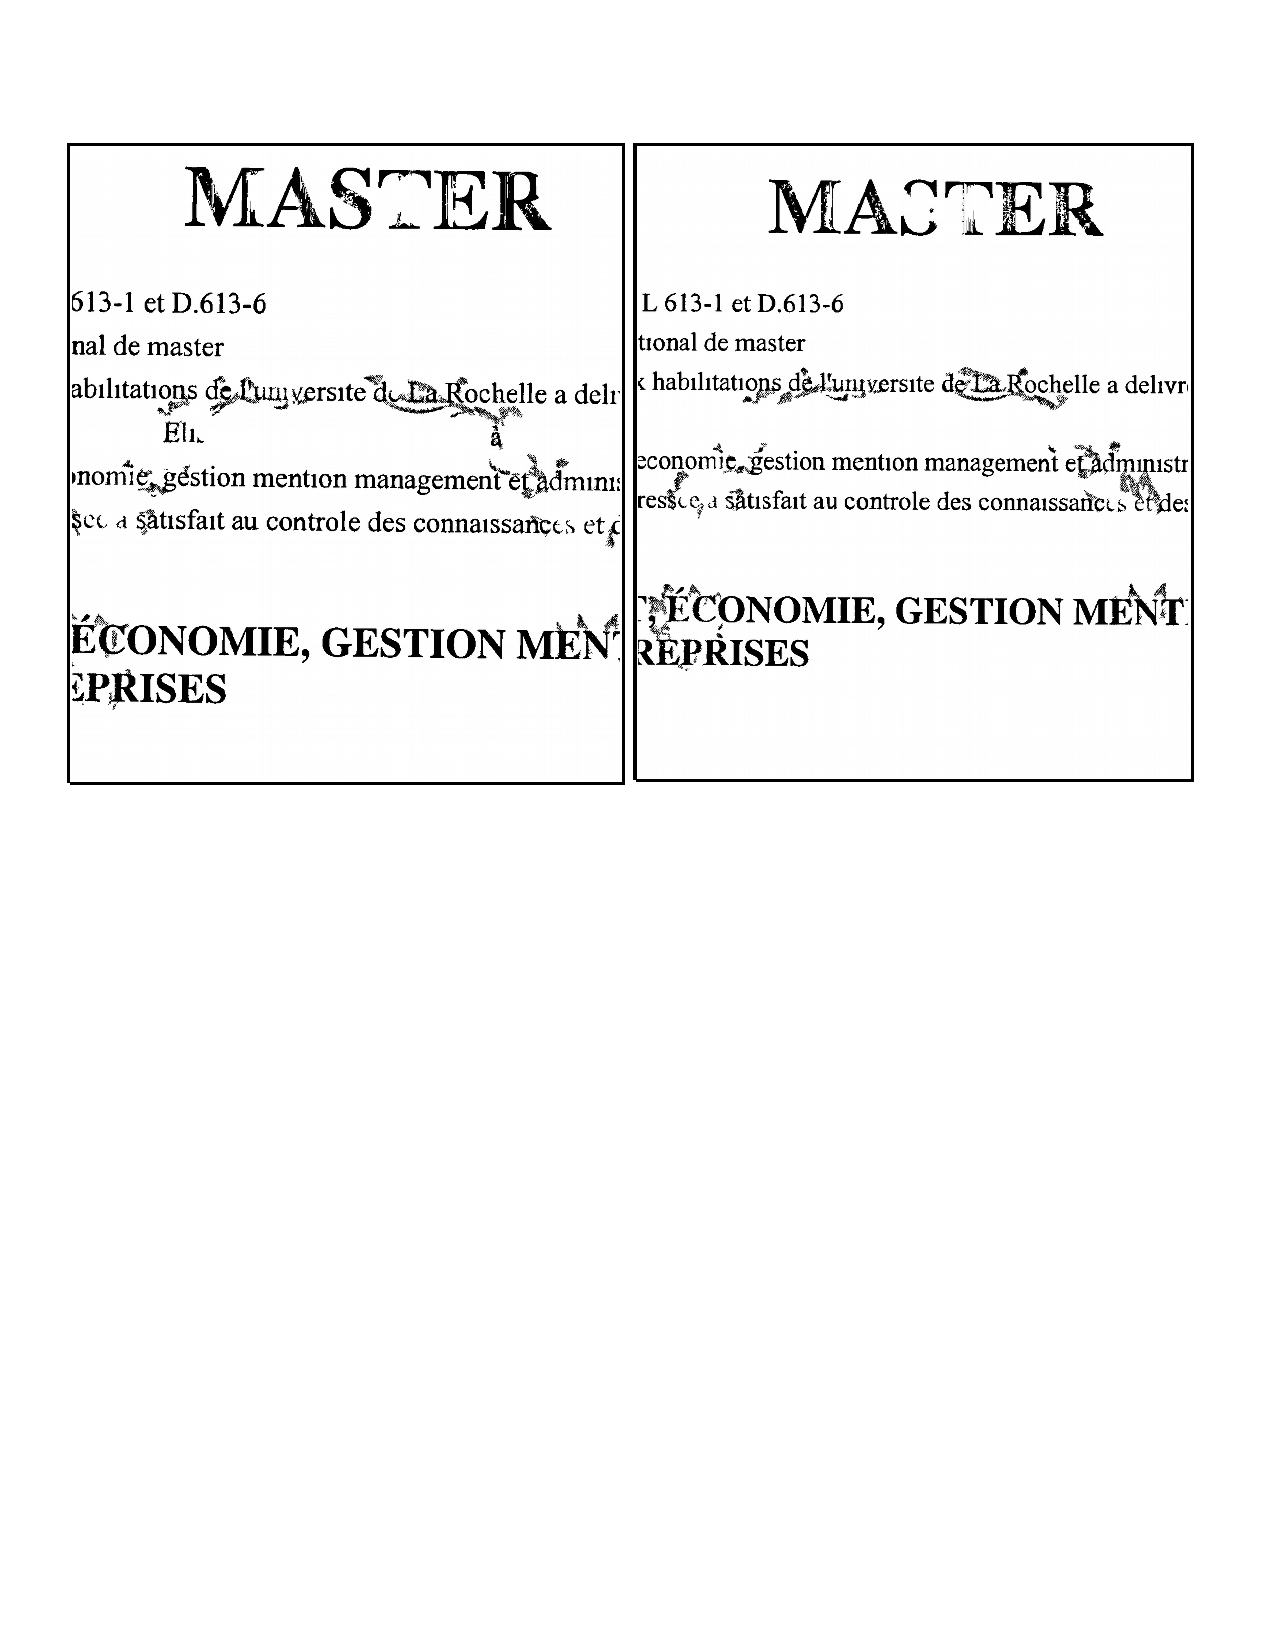
\includegraphics[trim = 2cm 15cm 2cm 2.4cm, clip,scale=0.24]{./images/bin_probs/mondal_probs.pdf}}
		\caption{}
		\label{image_text_19}
	\end{subfigure}	
	\begin{subfigure}[b]{0.32\textwidth}
		\centering \fbox{
\includegraphics[trim = 0cm 0cm 0cm 0cm, clip,scale=0.016]{./images/bin_probs/sspProbs.png}}
		\caption{}
		\label{image_text_20}
	\end{subfigure} 
	\caption[endProcess]{(a): The result of Savoula binarization (b) Some results of binarization by technique of Mondal et.al.\cite{Mondal2019}   (c) Binarization results by Jia et.al \cite{Jia2018}}
	\label{fig:imgBinari}
	%	\end{minipage}
\end{figure}

%\subsection{Results on DIBCO dataset} To examine the robustness, we also have applied our technique on $5$ DIBCO datasets (see Table \ref{tab:allResultStats}). It can be seen that even though for \textit{DIBCO-16} dataset, our method shows \textit{F-Measure} and \textit{DRD} values quite close to other best performing techniques, but for other DIBCO datasets, our approach doesn't perform at par. 
% 		 \subsection {Why it doesn't work on DIBCO dataset ?}  
%Although the proposed method performs quite well on diploma images but fails to perform better on DIBCO dataset whereas state of the art binarization techniques e.g. Savoula (see Fig. \ref{image_text_11}) and Dynamic window based (see Fig. \ref{image_text_12}) fails to perform on diploma images. 
%The possible reasons of the difference in performance in diploma and DIBCO dataset could be that DIBCO dataset contains handwritten and printed historical images, having non-uniform background, stains, faded and bleeding ink etc. The binarization techniques in literature are specially designed and parameters are adjusted by keeping in mind these image variations. Whereas our method is designed for diploma images, having the problem of decorated overlapping background. Moreover it can be seen in Fig. \ref{image_text_16} that the clustering was able to detect (sure and confused pixels) mostly all the correct text pixels. But due to the lower presence of sure text pixels around confused pixels, at the end many confused pixels fail to be qualified as text pixels ( see \ref{image_text_17}),  which finally decline the statistical accuracy.  
% 	    \begin{table*}[ht]
% 		\centering\small
% 		\caption{Result on University Diploma Dataset\label{tab:table1}}
% 		\begin{tabularx}{\linewidth}{XXX} 
% 			\toprule
% 			Dataset & Resolution &  \\
% 			\midrule
% 			Latency& Less than 10ms from user to server &   \\ 
% 			\bottomrule
% 		\end{tabularx}
% 	\end{table*}

\section{Conclusion}
In this paper, we have proposed a technique to remove background and to obtain texts from French university diplomas. Our proposed method performs satisfactory well on diploma images (see Table~\ref{table:binarizatonTime}). All experiments are done by using Intel i7-8850H CPU, 32 GB RAM (in C++ and Matlab R2018a). It can be concluded that the proposed approach performs satisfactorily well on diploma images compared to many other state of the art techniques.     

\section*{Acknowledgment}
This work is supported by the Region Nouvelle Aquitaine and European Union under the project ”Sécurisation et Authentification des Diplômes” in the ”programme opérationnel FEDER/FSE 2014-2020” (grant number P2017-BAFE-46). We highly thank the anonymous reviewers for their comprehensive reviews.  

\bibliographystyle{splncs04}
\bibliography{../../All_Biblios_Links/library.bib}
\end{document}
